\chapter{Vyhodnotenie a výsledky experimentu}


\section{Vyhodnotenie rôznych kombinácii alpha a beta parametrov}

The table \ref{table:1} is an example of referenced \LaTeX elements.
 
\begin{table}[h!]
\centering
\begin{tabular}{|c|c|} 
 \hline
 Parameter & Hodnota \\ 
 \hline\hline
 1 & 6  \\ 
 \hline
 2 & 7   \\
 \hline
 3 & 545  \\
 \hline
 4 & 545  \\
 \hline
 5 & 88 \\  
 \hline
\end{tabular}
\caption{Parametre RecSOM siete}
\label{table:1}
\end{table}


\begin{figure}[H]
    \centering
    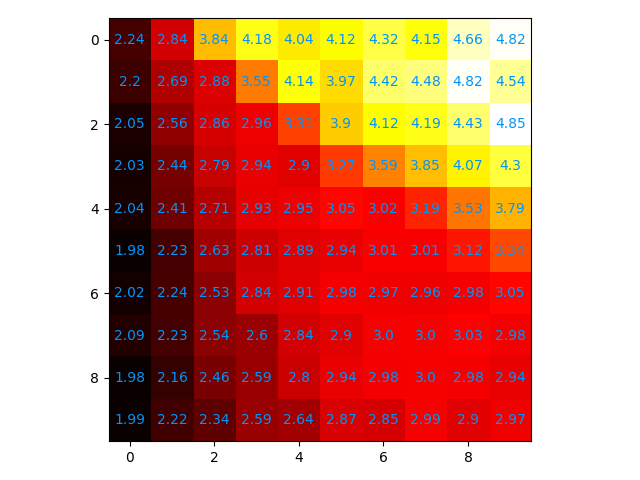
\includegraphics[width=8cm]{assets/recsom_abcd}
    \caption{Rec SOM results}
\end{figure}


\begin{table}[h!]
    \centering
    \begin{tabular}{|c|c|} 
     \hline
     Parameter & Hodnota \\ 
     \hline\hline
     1 & 6  \\ 
     \hline
     2 & 7   \\
     \hline
     3 & 545  \\
     \hline
     4 & 545  \\
     \hline
     5 & 88 \\  
     \hline
    \end{tabular}
    \caption{Parametre mSOM siete}
    \label{table:2}
\end{table}

\begin{figure}[H]
    \centering
    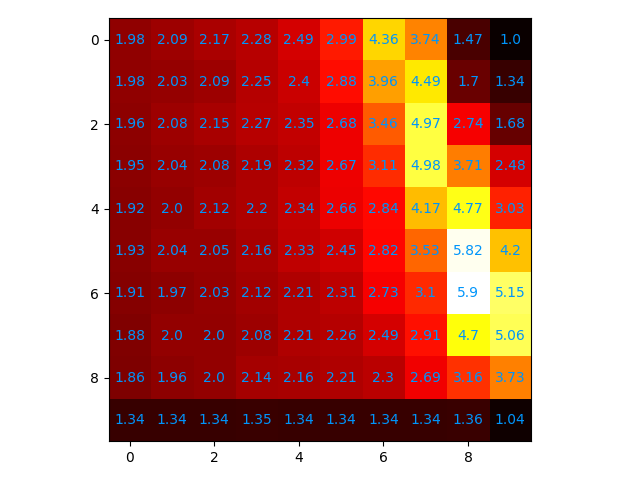
\includegraphics[width=8cm]{assets/msom_abcd}
    \caption{MSOM results}
\end{figure}


\begin{table}[h!]
    \centering
    \begin{tabular}{|c|c|} 
     \hline
     Parameter & Hodnota \\ 
     \hline\hline
     1 & 6  \\ 
     \hline
     2 & 7   \\
     \hline
     3 & 545  \\
     \hline
     4 & 545  \\
     \hline
     5 & 88 \\  
     \hline
    \end{tabular}
    \caption{Parametre leaky mSOM siete}
    \label{table:2}
\end{table}

\begin{figure}[H]
    \centering
    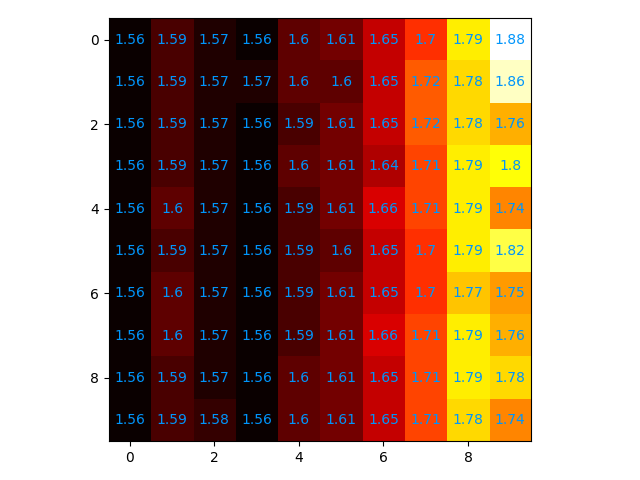
\includegraphics[width=8cm]{assets/leakymsom_abcd}
    \caption{Leaky MSOM results}
\end{figure}